\documentclass[a4paper,12pt]{article}
\usepackage[utf8]{inputenc}
\usepackage{graphicx} % Required for inserting images
\usepackage{hyperref}
\usepackage{amsmath}
\usepackage{amssymb}

\usepackage{dentitle}
\usepackage{personal}

\begin{document}

\title{Multimodal Transformers}
\author{Matheus Costa Monteiro}
\date{19 de maio de 2026}
\makedendentitle{PCS5029 - PLN com Redes Neurais Artificiais}{Relatório da Aula 12}{}

\section*{\textbf{O que é um Transformer Multimodal e como é feita a tokenização}}

Um Transformer Multimodal é uma arquitetura baseada em Transformers capaz de processar e relacionar informações provenientes de diferentes modalidades, como texto, imagem, áudio e vídeo. Em modelos multimodais modernos, uma estrutura comum consiste em utilizar um codificador específico para cada modalidade, por exemplo um encoder visual para imagens, um conector responsável por projetar essas representações para o mesmo espaço vetorial usado pelo modelo de linguagem, e um LLM que realiza o raciocínio e gera a resposta final \cite{yin2024survey}. Nesse contexto, a tokenização não se limita à divisão de texto em subpalavras, como ocorre em modelos puramente textuais. O texto continua sendo transformado em tokens discretos por um tokenizer, geralmente baseado em subword units, enquanto imagens podem ser divididas em patches ou processadas por um encoder visual que produz vetores representacionais. Esses vetores são então convertidos em \textit{tokens visuais}, alinhados dimensionalmente aos embeddings textuais por meio de um conector, como uma camada MLP, um Q-Former ou mecanismos de atenção cruzada \cite{yin2024survey}. Assim, o modelo recebe uma sequência conjunta composta por tokens textuais e tokens multimodais, permitindo que o Transformer aprenda relações entre linguagem e percepção visual ou sonora.

\section*{\textbf{Como criar um Transformer Multimodal}}

Existem duas estratégias principais para construir um Transformer Multimodal. A primeira, mais comum em modelos como LLaVA, BLIP-2 e Flamingo, parte de um LLM textual já pré-treinado e adiciona um módulo visual externo. Nessa abordagem, uma imagem é processada por um encoder visual, como CLIP ou ViT, que transforma a imagem em representações vetoriais contínuas. Em seguida, um conector aprende a projetar essas representações para o espaço de embeddings do LLM. Dessa forma, o modelo de linguagem passa a receber, além dos tokens textuais, também tokens ou vetores derivados da imagem. Essa abordagem é eficiente porque reaproveita modelos já treinados, reduz o custo computacional e permite adaptar LLMs textuais para tarefas multimodais \cite{yin2024survey}.

A segunda estratégia, exemplificada pelo Chameleon, é mais unificada e consiste em treinar um modelo \textit{mixed-modal} desde o início. Nesse caso, texto e imagem são ambos convertidos em tokens discretos e inseridos em uma única sequência autoregressiva. O texto é tokenizado por um tokenizer BPE, enquanto a imagem é convertida por um tokenizador visual em uma sequência de tokens de imagem. No Chameleon, uma imagem de $512 \times 512$ pixels é representada por $1024$ tokens discretos escolhidos a partir de um codebook visual de tamanho $8192$ \cite{chameleon2024}. Assim, uma sequência de entrada pode conter texto, tokens especiais de início e fim de imagem, tokens visuais e novamente tokens textuais, todos processados pelo mesmo Transformer.

\begin{figure}[htbp]
    \centering
    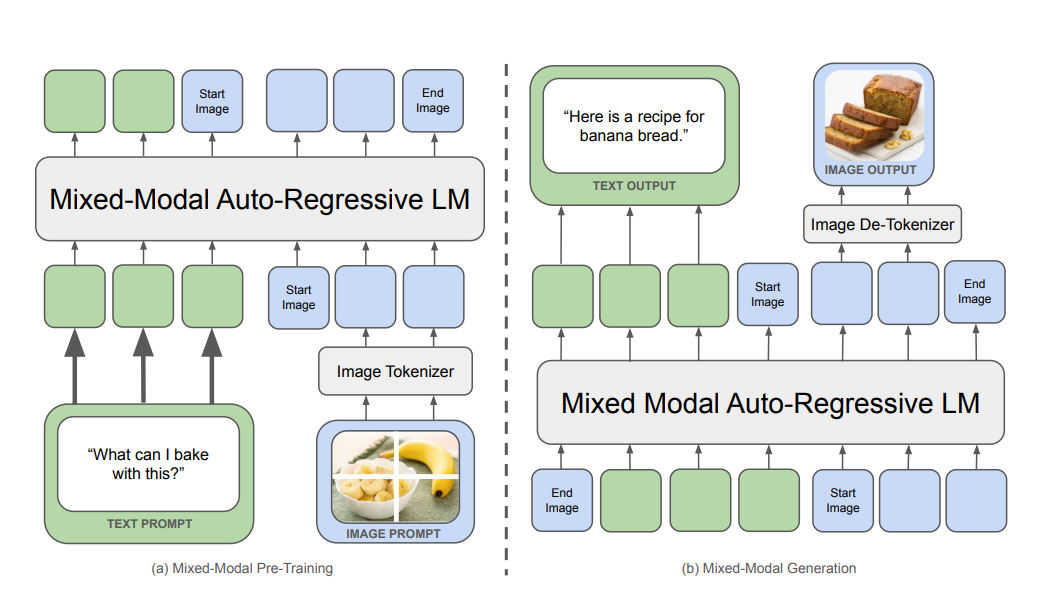
\includegraphics[width=\textwidth]{unified-multimodal-transformer.png}
    \caption{Arquitetura geral do Chameleon como modelo autoregressivo multimodal. À esquerda, o modelo recebe texto e imagem tokenizados durante o pré-treinamento. À direita, o mesmo modelo gera texto e imagem de forma intercalada. Adaptado de \cite{chameleon2024}.}
    \label{fig:chameleon-mixed-modal}
\end{figure}

A Figura~\ref{fig:chameleon-mixed-modal} ilustra a principal diferença entre um MLLM baseado em conector visual e um modelo \textit{early-fusion}. Em vez de processar a imagem em um encoder externo e depois adaptar suas representações para o LLM, o Chameleon transforma a imagem em tokens discretos e os coloca na mesma sequência dos tokens textuais \cite{chameleon2024}. Isso permite que o modelo opere como um único Transformer autoregressivo capaz de prever o próximo token, seja ele textual ou visual. Em outras palavras, a imagem passa a ser tratada como uma sequência simbólica, de forma análoga à linguagem natural.

A criação de um Transformer Multimodal envolve, portanto, quatro decisões centrais. Primeiro, é necessário definir como cada modalidade será representada: texto como subpalavras, imagens como patches, embeddings visuais ou tokens discretos, áudio como espectrogramas ou tokens acústicos, e assim por diante. Segundo, é preciso escolher a forma de fusão entre modalidades. Na fusão tardia, cada modalidade é processada separadamente e combinada depois; na fusão inicial, como no Chameleon, todas as modalidades já entram desde o início como uma sequência compartilhada de tokens \cite{chameleon2024}. Terceiro, é necessário treinar o modelo com dados multimodais, como pares imagem-texto, documentos intercalados com imagem e texto, dados de instrução visual e exemplos de geração multimodal. Quarto, é preciso alinhar o modelo para seguir instruções humanas, normalmente por meio de \textit{supervised fine-tuning} e, em alguns casos, técnicas de alinhamento por preferência \cite{yin2024survey}.

A principal vantagem da abordagem com encoder e conector é a praticidade: ela permite transformar rapidamente um LLM textual em um modelo capaz de compreender imagens. A principal vantagem da abordagem \textit{early-fusion} é a generalidade: o modelo aprende a tratar texto e imagem como partes de uma mesma linguagem, podendo compreender e gerar documentos com texto e imagens intercalados \cite{chameleon2024}. Por outro lado, essa abordagem é mais difícil de treinar, pois modalidades diferentes possuem distribuições estatísticas distintas e podem causar instabilidades no treinamento. Por isso, o Chameleon introduz técnicas específicas de estabilidade, como QK-Norm, regularização por \textit{z-loss} e mudanças na ordem das normalizações internas do Transformer \cite{chameleon2024}.

Em síntese, criar um Transformer Multimodal significa transformar diferentes modalidades em representações compatíveis, combiná-las em uma arquitetura Transformer e treinar o modelo para prever saídas condicionadas a múltiplos tipos de entrada. A diferença fundamental entre os modelos está em onde ocorre a fusão: modelos baseados em encoder e conector fazem a fusão depois que cada modalidade já foi processada separadamente, enquanto modelos \textit{early-fusion} fazem a fusão logo no nível dos tokens. Essa distinção é central para entender a evolução recente dos MLLMs.

\begin{thebibliography}{9}

\bibitem{yin2024survey}
YIN, Shukang et al.
\textit{A survey on multimodal large language models}.
National Science Review, v. 11, n. 12, nwae403, 2024.
DOI: \href{https://doi.org/10.1093/nsr/nwae403}{10.1093/nsr/nwae403}.

\bibitem{chameleon2024}
CHAMELEON TEAM.
\textit{Chameleon: Mixed-Modal Early-Fusion Foundation Models}.
arXiv preprint arXiv:2405.09818, 2024.

\end{thebibliography}

%\bibliographystyle{abntex2-num}
%\bibliographystyle{abntex2-alf}
%\bibliography{references}

\end{document}